\clearpage
\section{Matching mit dem Standardmodell}

  Abschließend soll nun diskutiert werden, inwieweit die Einführung der dQCD 
  Abweichungen von Standardmodell bewirkt. Sei $M$ eine charakteristische 
  Massenskala des joint-Sektors. Da diese Teilchen QCD-Ladung tragen, ist 
  $M > \mathcal{O}(100\,\text{GeV})$, sonst wären diese in aktuellen 
  Experimenten bereits gefunden worden 
  \cite{Scale_of_dark_QCD}\cite{Becciolini:2014lya}. In 
  \cite{Becciolini:2014lya} und \cite{Sannino} wird das Verhältnis 
  der differenziellen Wirkungsquerschnitte von 3- und 2-Jet Zerfällen als 
  sinvolle Observable für hochenergie QCD eingeführt
  und daran argumentiert, dass 
  die \textit{Partonverteilungsfunktionen (PDF)} der neuen Teilchen sowie die 
  Auswirkungen auf die PDFs der SM Teilchen vernachlässibar sind. Sie zeigen 
  weiter, dass solche Verhältnisse nicht sensitiv auf die Gluon PDF sind und 
  schließen daraus, dass das Laufen von $\alpha_\text{QCD}$ den wichtigsten 
  Einfluss auf solche Observablen hat. Aus diesem Grund wird nun das Laufen 
  von $\alpha_\text{QCD}$ im SM mit $\alpha_1$ aus der \QCDxdQCD verglichen. 
  
  Die bisher untersuchten $\beta$-Funktionen gelten nur für Energien oberhalb 
  der Massenskala $M$ der schwersten neuen Teilchen \cite{Becciolini:2014lya}. 
  Man kann nun bis zur Energieskala $Q$ eine effektive Theorie einführen, bei 
  der schwere Teilchen mit Massen $m > Q$ ausintegriert werden. 
  Durch dieses Vorgehen ist es möglich, die volle \QCDxdQCD bei $Q$ zu 
  entkoppeln und das bekannte Verhalten der SM QCD zu erhalten 
  \cite{Bednyakov2015262}. Für das dunkle Materie Szenario berechnen Bai und 
  Schwaller eine Entkopplungsskala von $Q \gtrsim 500\,\text{GeV}$. An dem 
  entsprechenden Phasenraumdiagramm in Abbildung \ref{fig:messbarkeit:IR-Fix}
  ist zu sehen, dass in ihrem Szenario $\alpha^{*2}$ und $\alpha^{*3}$ als 
  interessante UV-Fixpunkte in Frage kommen. Als Entkopplungsskala werden die 
  CMS Daten $Q=474\,\text{GeV}$ mit 
  $\alpha_\text{QCD}^\text{exp}(Q)=0.0936 \pm 0.0041$ verwendet
  \cite{Chatrchyan:2013txa}. Die Entkopplungsskala ist aus theoretischer Sicht 
  beliebig, die Wahl $ Q \approx M$ ist jedoch die üblichste und anschaulichste
  Wahl. Im Folgenden 
  wird erklärt, wie in einem Modell mit zwei Kopplungskonstanten ein Fixpunkt 
  extrapoliert werden kann, danach wird diese Methode auf einige der gefundenen 
  Modelle angewandt.
  \begin{figure}
 \centering
 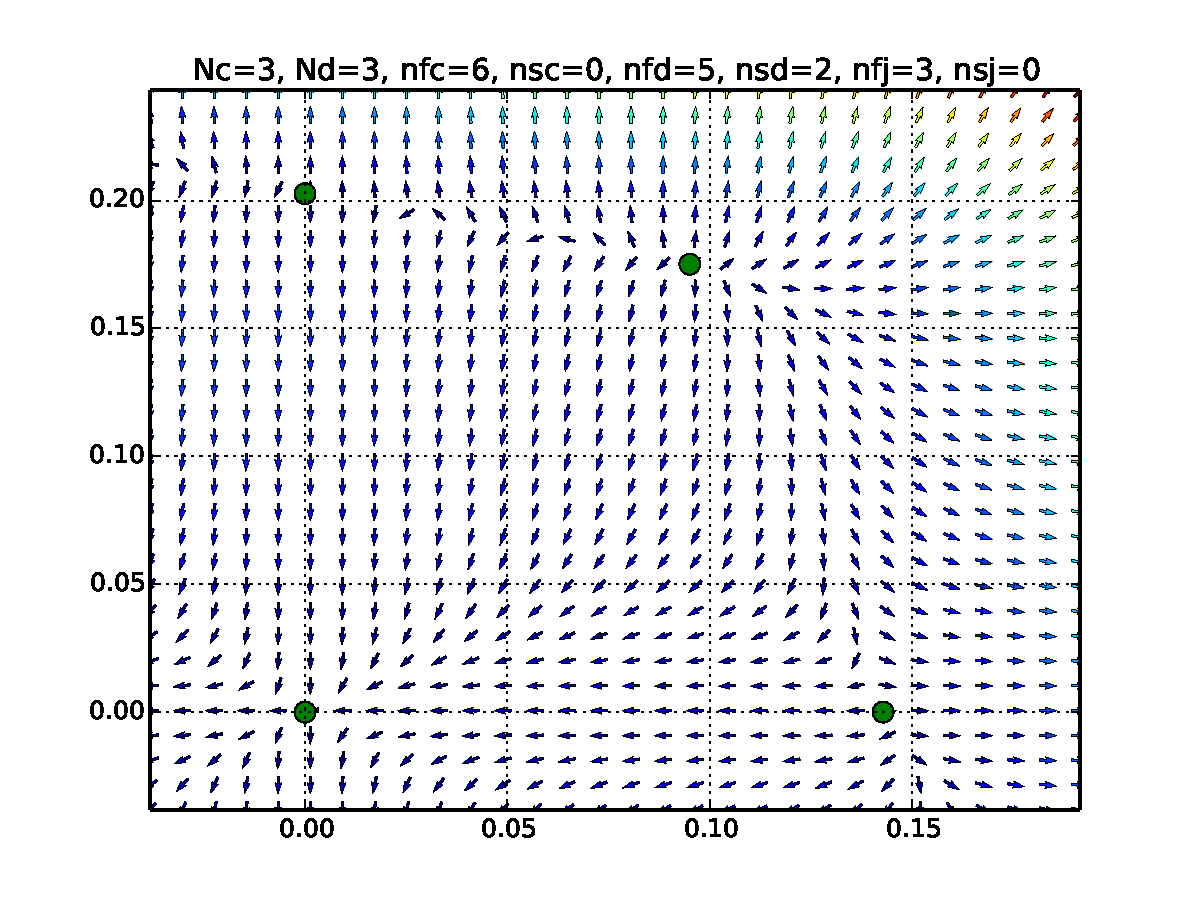
\includegraphics[scale=0.7]{abschnitte/messbarkeit/fig/RG_flow3_3_6_0_5_2_3_0.pdf}
 \caption{Phasenraumdiagramm mit wechselwirkendem IR-Fixpunkt, mit SM+$\Nd=3$, $\nfd=5$, $\nsd=2$ und $\nfj=3$.}
 \label{fig:messbarkeit:IR-Fix}
\end{figure}

  
  
  \subsection{Extrapolation eines Fixpunktes}
    Um das UV-Verhalten einer $\beta$-Funktion mit den bisher gemessenen Werten 
    für die Kopplungskonstanten im SM vergleichen zu können, ist es notwendig 
    die kritische Hyperfläche eines Fixpunktes auch in einem Bereich zu kennen, 
    der zu groß für eine Taylorentwicklung geringer Ordnung ist. Das Auffinden 
    der kritischen Hyperfläche ist insbesondere für höherdimensionale Probleme 
    analytisch kaum möglich und daher eine numerische Aufgabe. Stehen nun 
    $n$ Messwerte an der selben Renormierungsskala 
    $\mu_0$ zur Verfügung und gibt es einen Punkt $\alpha_0\in\Mc$ der diese 
    enthält, dann sind alle Kopplungskonstanten $\alpha(\mu)$ bis auf 
    $(\dim (\Mc)-n)$ freie Parameter festgelegt\footnote{Für $n\geq \dim(\Mc)$ 
    also eindeutig.} und laufen in den Fixpunkt hinein. Existiert so ein 
    $\alpha_0\in\Mc$ nicht, kommt der untersuchte Fixpunkt für ein asymptotic 
    safety Szenario nicht in Frage. 

  
    Ein besonderer Vorteil einer Erweiterung $G \to G_1\times G_2$ ist die 
    Möglichkeit einen UV-Fixpunkt eindeutig extrapolieren zu können, da die 
    kritische Hyperfläche die Dimension $\dim(\alpha^*)=0$, 
    $\dim(\text{Trajektorie})=1$ oder $\dim(\text{Phasenraum})=2$ hat. Im 
    ersten Fall, $\dim \Mc=0$ besteht sie nur aus dem Fixpunkt selbst, 
    dieser Fall ist also eher als eine mathematische, triviale Lösung zu 
    betrachten, die keine physikalische Bedeutung im Sinne laufender 
    Kopplungskonstanten hat. Im Fall $\dim \Mc =2$ besteht sie aus dem gesamten 
    Phasenraum. Weil in diesem Fall jede Trajektorie in den Fixpunkt 
    hineinläuft kann keine Vorhersage für die Größen der Kopplungskonstanten 
    gemacht werden, dafür ist aber das UV-Verhalten von dem Startwert 
    $\left(\alpha_1(t_0),\alpha_2(t_0)\right)$ unabhängig. Wie bereits 
    gezeigt ist dieser Fall hier nicht möglich. Der für die 
    Extrapolation interessanteste Fall ist also $\dim \Mc = 1$, da die 
    UV-Hyperfläche dann aus zwei Trajektorien 
    $s^{+/-}:(0,\infty)\to \mathbb{R}^2$ besteht\footnote{Jeweils eine in, eine 
    entgegen der Richtung des attraktiven Eigenvektors.} und deshalb 
    eindeutige Wertepaare $(\alpha_1(t),\alpha_2(t))$ vorhersagt. Wenn eine 
    Kopplungskonstante (o.E.) $\alpha_1(t_0)$ bei einer Renormierungsskala 
    $t_0$ bekannt ist, und unter der Annahme, dass der Fixpunkt für 
    $t\to\infty$ erreicht wird, ist somit auch $\alpha_2(t_0)$ sowie das 
    gesamte Verhalten beider Kopplungskonstanten bekannt.
    
    Für die Extrapolation werden außerdem die folgende Beobachtungen ausgenutzt.
    \begin{enumerate}
     \item Eine Trajektorie, welche in einen Sattelpunkt hineinläuft, ist 
     gleichzeitig eine Separatrix, d.h. sie teilt den Phasenrau in Gebiete mit 
     qualitativ unterschiedlichem  Verhalten für $t \to \infty$.
     \item Ein Sattelpunkt und ein attraktiver Fixpunkt sind mit einer 
     Separatrix verbunden, ebenso ist ein Sattelpunkt mit einem repulsiven 
     Fixpunkt mit einer Separatrix verbunden, sofern die Fixpunkte existieren 
     und in der Nähe des Sattelpunktes liegen. 
    \end{enumerate}

    Da das gesuchte $\Mc$ folglich immer eine Separatrix ist, kann wie folgt 
    verfahren werden. Zunächst werden zwei Gebiete $L$ und $R$ definiert, die 
    zu qualitativ verschiedenen Trajektorien führen. Beispielsweise lassen sich 
    oft Abschätzungen der Art finden: Wenn es 
    ein $t_1$ gibt mit
    \begin{equation}
     \alpha_j(t_1) > \max \left\{ \left. \alpha^{*i}_j \right|\text{alle 
     Fixpunkte } 
     \alpha^{*i}\right\} \quad ,
    \end{equation}
    dann kann der gewünschte Fixpunkt nicht mehr für $t>t_1$ erreicht werden.
    Am Fixpunkt wird eine Orthonormalbasis $\{f_1,f_2\}$ gewählt\footnote{Der 
    Einfachheit halber kann die Basis aus Eigenvektoren oder die 
    $\alpha_{1,2}$-Achsen gewählt werden, sofern dies 
    zu keinen numerischen Schwierigkeiten führt.}
    und der Phasenraum in Ebenen mit Abstand $\epsilon$ 
    eingeteilt, die nullte Ebene geht dabei durch den Fixpunkt. Rekursiv werden 
    dann
    \begin{equation}
     s^{L/R}[n+1] = s^{L/R}[n] + \epsilon f_1 + d^{L/R} \delta f_2 
    \end{equation}
    definiert. Für festes $\delta$ wird $d^{L/R}$ so eingestelle, dass die 
    Trajektorie 
    mit Anfangswert $s^L[n+1]$ in den Bereich $L$ hineinläuft, analog für 
    $R$. 
    Mit
    \begin{equation}
    s^L[0]:=\alpha^*-\nicefrac{\delta}{2}  f_2\quad \text{und} \quad
    s^R[0]:=\alpha^*+\nicefrac{\delta}{2} f_2
    \end{equation}
    ergibt sich so ein Schlauch $\left(s^{L}[n],s^R[n] \right)_{n=0,1,\ldots}$ 
    der Breite 
    $\delta$, der die Separatrix beinhaltet.
    Näherungsweise wird nun 
    \begin{equation}
     \alpha[n] := \frac{s^L[n]+s^R[n]}{2}
    \end{equation}
    definiert und so sortiert, dass $\alpha[0]\simeq\alpha(t_0)$ und 
    $\alpha[n]\rightarrow \alpha^*$ für steigendes $n$.
    Die entsprechende RG-Zeit $t$ wird dann über 
    \begin{equation}
     t[n+1]= \frac{\left\lVert \alpha[n+1]-\alpha[n] \right\rVert}{\left\lVert 
     \beta(\alpha[n])\right\rVert} + t[n]
    \end{equation}
    mit $t[0]=t_0$ berechnet.
    
    Um die so erhaltenen laufenden Kopplungen mit dem Standardmodell zu 
    vergleichen wird noch die SM QCD Kopplung in $\mathcal{O}(\alpha^3)$ 
    berechnet. Dies geschieht implizit über 
    \begin{equation}
     F(\alpha(t)) = t-t_0 +F(\alpha(t_0)) \label{eq:messbarkeit:SM-running}
    \end{equation}
    mit 
    \begin{equation}
     F(\alpha) := \int \left(\beta_\text{QCD}\right)^{-1} \,\,\, 
     \text{d}\,\alpha
     = \int \left(X_1 \alpha^2 +Y_1 \alpha^3\right)^{-1} \,\,\, \text{d}\,\alpha
     = \frac{Y_1}{X_1^2} \ln\left(\frac{\alpha Y_1+X_1}{\alpha}\right) -
     \frac{1}{\alpha X_1}
    \end{equation}
    und $\nfj=\nsj=0$. Der Einfachheit halber wird $\Lambda_0 = Q$ gewählt, 
    sodass $t_0=0$ und $\alpha(0)$ die Startwerte sind.
    
    
  \subsection{Extrapolation von $\alpha^{*3}$} \label{extrapol_afix3}
    \begin{figure}
 \centering
 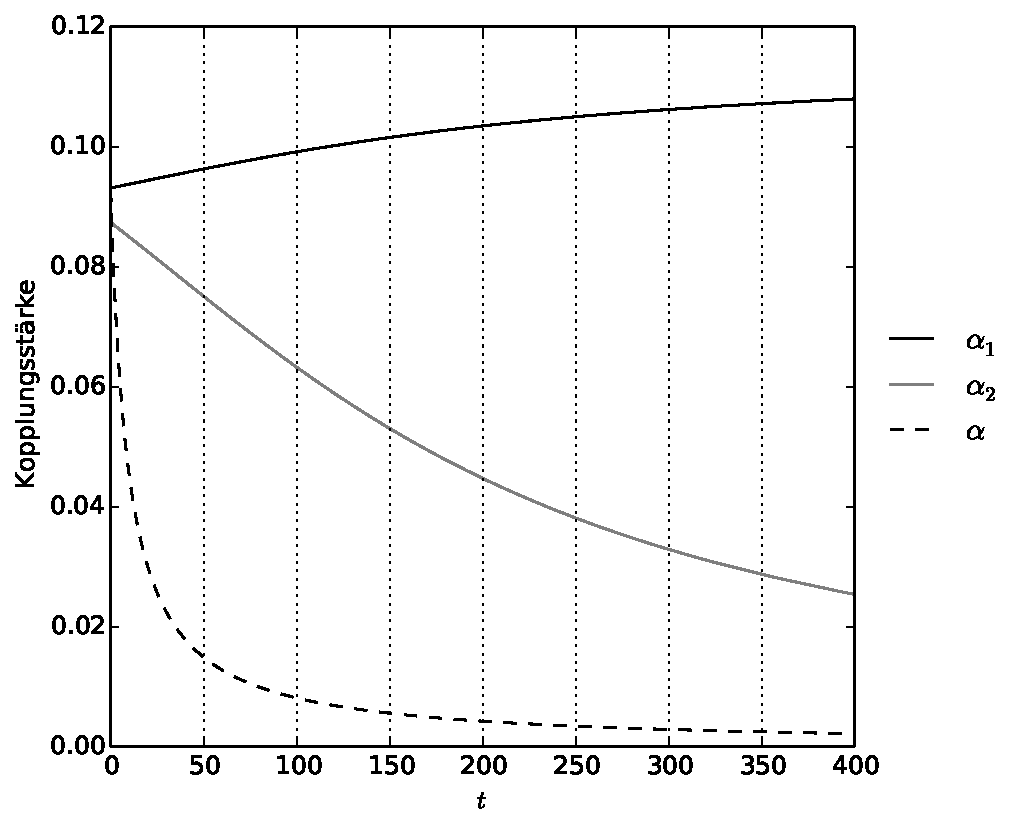
\includegraphics[scale=0.7]{Python/plots/alpha_running/Kopplungen1_afix3.pdf}
 \caption{Die laufenden Kopplungen $\alpha_1$, $\alpha_2$ und $\alpha$ zum Fixpunkt 
 $\alpha^*_\text{tw1}$ für die Parameter  $(\Nc,\Nd,\nfc,\nsc,\nfd,\nsd,\nfj,\nsj)=(3,3,6,1,6,0,3,0)$.}
 \label{fig:messbarkeit:afix3}
\end{figure}

    
    Im Folgenden sind $\alpha_1(t)$ und $\alpha_2(t)$ die Kopplungskonstanten 
    der \QCDxdQCD entlang auf der UV-Hyperfläche, während $\alpha(t)$ die 
    SM QCD Kopplungskonstante darstellt.
    
    Wegen 
    \begin{equation}
     e_1 = \begin{pmatrix}
            1 \\ 0
           \end{pmatrix} \quad , \quad
    e_2 \propto \begin{pmatrix}
            -\frac{Z_1}{Y_1} \\ 1
           \end{pmatrix} \quad , \quad
    \lambda_1 >0
    \end{equation}
    und $Z_1>0$, $Y_1>0$ ist $\alpha_1$ steigend, während $\alpha$ als SM 
    Kopplung für hohe Energien fällt, wie in Abbildung 
    \ref{fig:messbarkeit:afix3} zu sehen ist. Aus $\alpha$-sensiblen 
    Observablen sollte es hier möglich sein, entsprechend hohe Grenzen an 
    die neuen Teilchenmassen $M$ zu setzen.
    
  \subsection{Extrapolation von $\alpha^{*2}$}
    \begin{table}
  \centering
 \begin{tabular}{c|cccccccc}
  \toprule
  \midrule
    & $\Nc$	&$\Nd$	&$\nfc$	&$\nsc$	&$\nfd$	&$\nsd$	&$\nfj$	&$\nsj$ \\
 \midrule
 a	&$3$	&$2$	&$6$	&$0$	&$3$	&$0$	&$1$	&$0$	\\
 b	&$3$	&$3$	&$6$	&$0$	&$9$	&$0$	&$1$	&$0$	\\
 c	&$3$	&$3$	&$6$	&$0$	&$10$	&$0$	&$2$	&$0$	\\
 d	&$3$	&$4$	&$6$	&$0$	&$17$	&$0$	&$1$	&$0$	\\
 e	&$3$	&$5$	&$6$	&$0$	&$24$	&$0$	&$1$	&$0$	\\
 \midrule
 \bottomrule
 \end{tabular}
\caption{Die Teilcheninhalte der Modelle a bis e.}
\label{tab:messbarkeit:modelle}
\end{table}

    \begin{figure}[h]
  \centering
  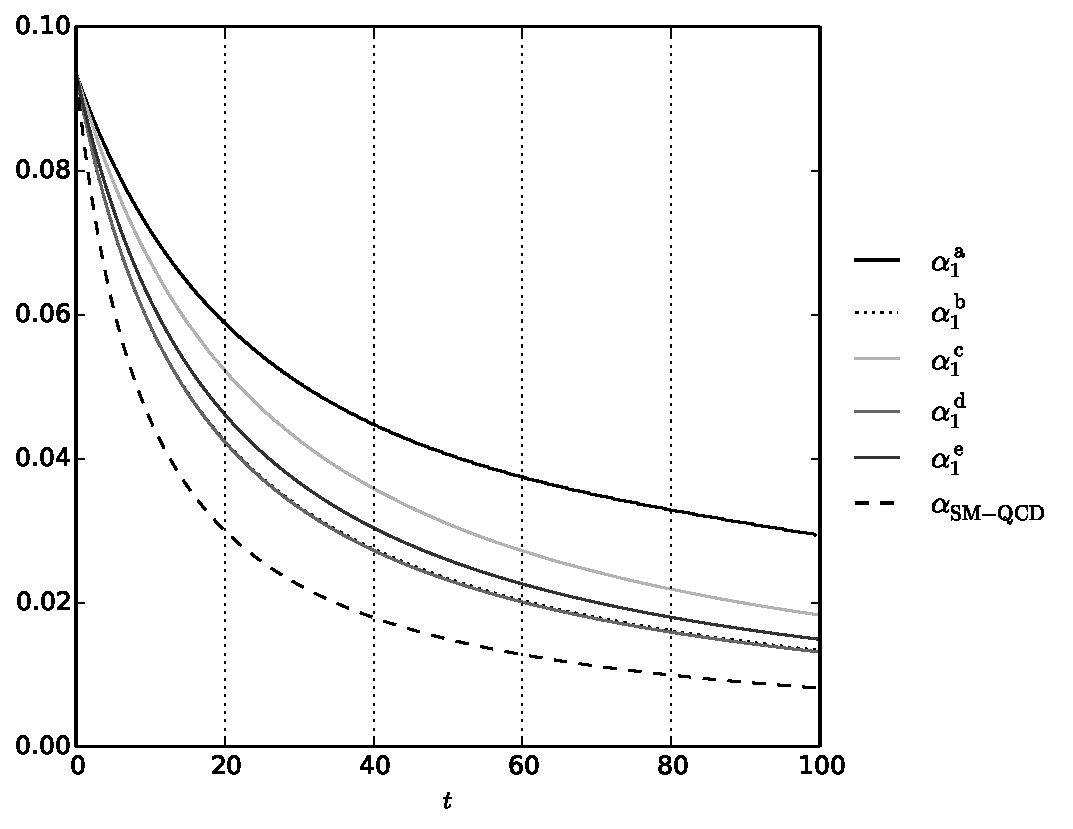
\includegraphics[scale=0.7]{Python/plots/alpha_running/Kopplungen1_her.pdf}
  \caption{Die laufende Kopplung $\alpha_\s$ zum Fixpunkt $\alpha^*_\text{tw2}$ für die  Modelle a bis e sowie 
  das SM $\alpha_\text{QCD}$.}
  \label{fig:messbarkeit:alpha_running_afix2}
\end{figure}

\begin{figure}
  \centering
  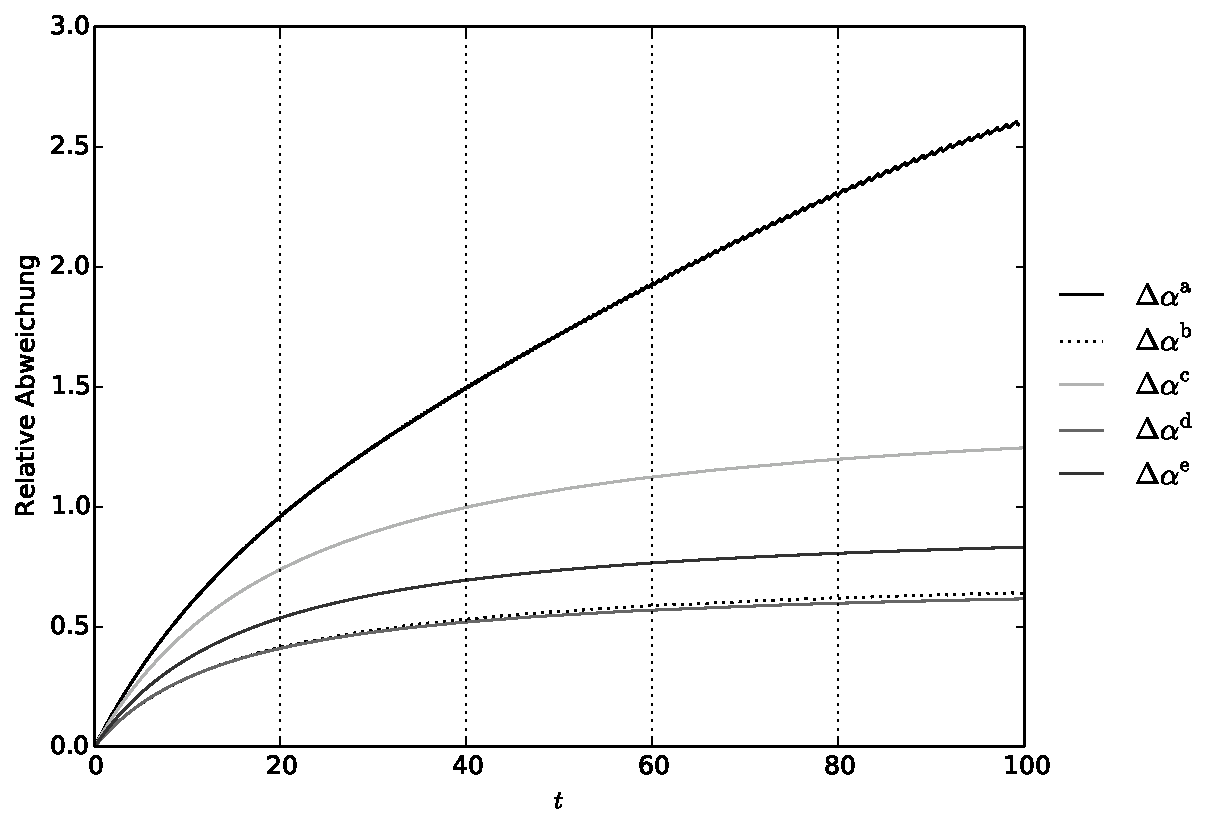
\includegraphics[scale=0.7]{Python/plots/alpha_running/relative_deviation_her.pdf}
  \caption{Die relative Abweichung von $\alpha_\s$ in \QCDxdQCD von $\alpha_\text{QCD}$  
  im SM für die Modelle a bis e.}
  \label{fig:messbarkeit:relative_deviation}
\end{figure}

    Die laufenden Kopplungen für die Beispielmodelle a bis e (vgl. Tabelle 
    \ref{tab:messbarkeit:modelle}) sind in Abbildung 
    \ref{fig:messbarkeit:alpha_running_afix2} zu sehen, die relativen 
    Abweichungen $\Delta \alpha_1 = (\alpha_1-\alpha)/\alpha$ in Abbildung 
    \ref{fig:messbarkeit:relative_deviation}. Hier verhält sich $\alpha_1$ 
    qualitativ wie $\alpha$, die relativen Abweichungen bei 
    $\mu = 1\,\text{TeV} \sim t \approx 0.746$ betragen hier 
    $\Delta \alpha \approx 3 \text{-} 5 \, \%$, bei $\mu = 2 \,\text{TeV} \sim t 
    \approx 1.439$ bereits $\Delta \alpha \approx 6\text{-}10 \, \%$ und liegen 
    damit im Bereich der erwarteten Messungenauigkeiten 
    (vgl. \cite{Bednyakov2015262}).
    
  \subsection{Extrapolation von $\alpha^{*4}$}
    \begin{figure}[h]
 \centering
 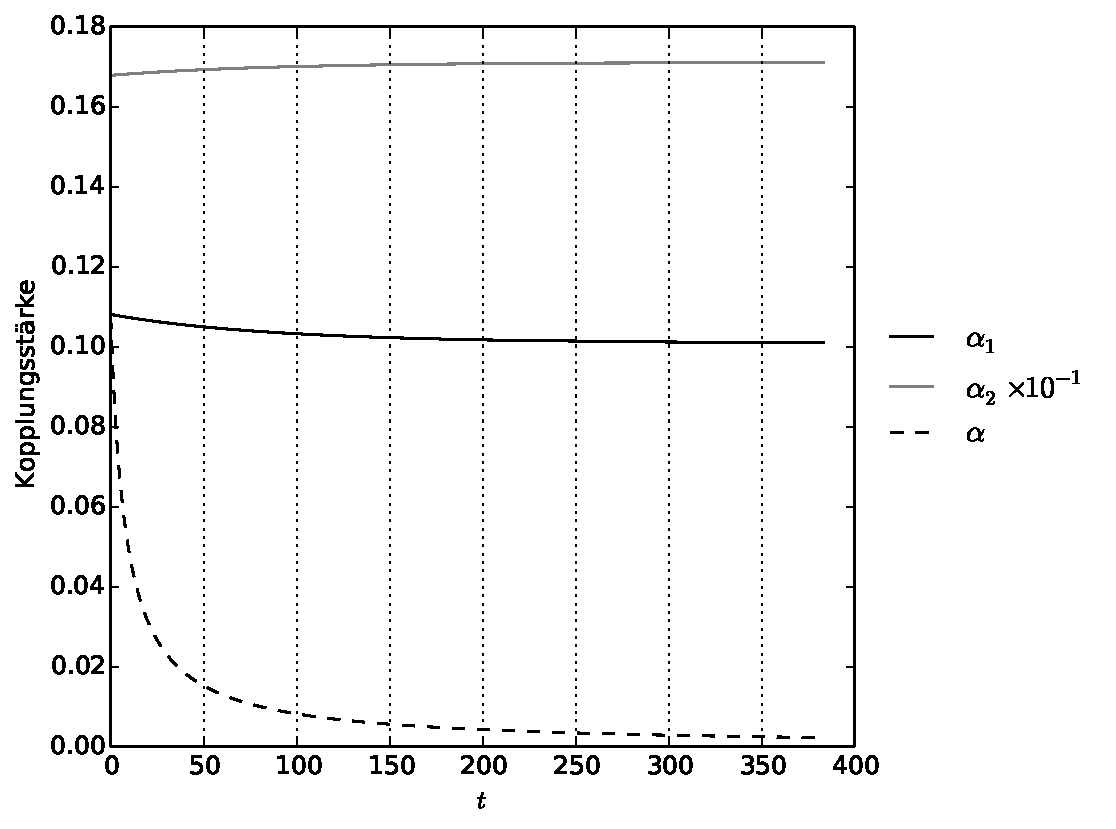
\includegraphics[scale=0.7]{Python/plots/alpha_running/Kopplungen1_afix4.pdf}
 \caption{Die laufenden Kopplungen $\alpha_\s$ und $\alpha_\text{QCD}$ zum Fixpunkt $\alpha^*_\text{vw}$ für die Parameter $(\Nc,\Nd,\nfc,\nsc,\nfd,\nsd,\nfj,\nsj)=(3,2,6,0,0,1,0,9)$.}
 \label{fig:messbarkeit:afix4}
\end{figure}

    Um ein SM-ähnliches Verhalten zu erzeugen muss 
    $\alpha_1(0)>\alpha_1^{*4}$. Der kleinste Wert für $\alpha_1^{*4}
    \approx 0.1007$ wird für $\text{SM}+(\Nd=2, \nsd=1,\nsj=9)$ angenommen. Da 
    $\alpha$ monoton fallend ist, muss die Entkopplungsskala $Q$ entsprechend 
    niedrig gewählt werden, um mit experimentellen Befunden im Einklang zu sein 
    jedoch mindestens auf die $t$-Masse $Q \approx 173.21 \, \text{GeV}$ 
    \cite{PDG:top}.
    Mit \eqref{eq:messbarkeit:SM-running} wird 
    ausgehend von der bekannte Kopplungskonstanten 
    $\alpha(M_Z=91.1876)=0.1185$ \cite{PDG:constants} mit effektiv 
    $5$ SM-Fermionen $\alpha(Q)=0.1081$ berechnet. In Abbildung 
    \ref{fig:messbarkeit:afix4} ist der weitere Verlauf für hohe Energien zu 
    sehen. Nach Konstruktion verhalten sich $\alpha_1$ und $\alpha$ qualitativ 
    ähnlich, da $\alpha_1^{*4}$ jedoch sehr nah am Startwert liegt ist hier 
    bei $1\,\text{TeV}$ die relative Abweichung bereits 
    $\Delta \alpha \approx 20 \%$.
    
    Eine Extrapolation von $\alpha^{*4}$ in Richtung kleiner QCD-Kopplungen 
    ist ebenfalls möglich, 
    verhält sich jedoch wie die Extrapolation von $\alpha^{*3}$ (vgl. 
    \ref{extrapol_afix3}).
    
    
   